\chapter{Metodologia}

A partir das 4 macro atividades do processo de medição: Estabelecer e manter compromisso com o processo de medição, Planejar o processo de medição, Executar o processo de medição e Avaliar o processo de medição, foram descritas outras atividades referentes a essas.

\begin{figure}[!htp]
		\centering
		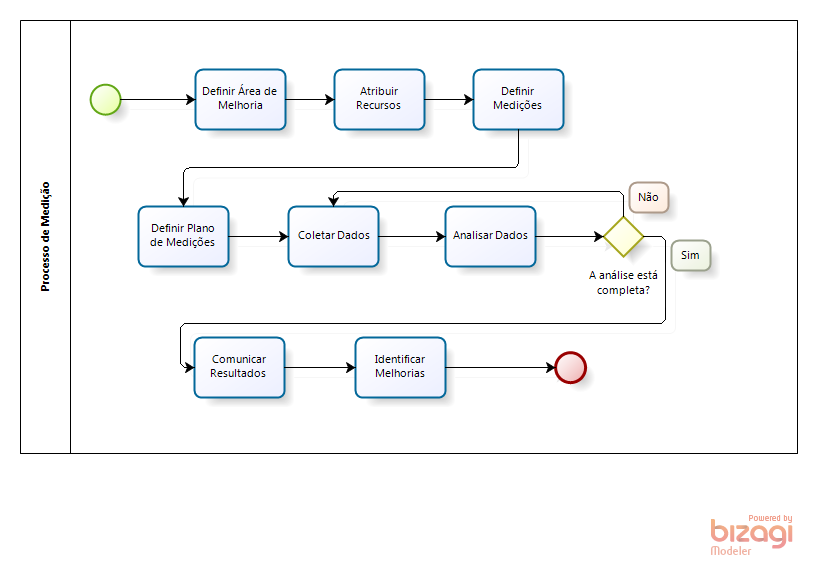
\includegraphics[scale=0.55]{figuras/medicao}
		\label{img:processo}
		\caption{Visão geral do Processo de Medição}
\end{figure}

\section{Descrição das Atividades}

\begin{enumerate}
\item Estabelecer e manter compromisso com o processo de medição

\textbf{Definir Área de Melhoria:} Esta atividade consiste em definir um projeto, bem como a área a ser realizada o processo de medição e em definir o escopo.

\textbf{Atribuir Recursos:} Atividade responsável por alocar recursos com competência  para a execução do processo.

\item Planejar o processo de medição

\textbf{Definir Medições:} Esta atividade consiste em definir as métricas a serem coletadas durante o processo.

\textbf{Definir Plano de Medições:} Esta atividade consiste em estabelecer como será executada a coleta e análise de métricas.

\item Executar o processo de medição

\textbf{Coletar Dados:} Atividade responsável pela coleta de métricas previamente definidas.

\textbf{Analisar Dados:} Esta atividade consiste na análise das métricas coletadas, a fim de que obtenha-se um entendimento do impacto dessas métricas no projeto.

\textbf{Comunicar Resultados:} Esta atividade consiste na descrição da análise feita sobre as métricas.

\item Avaliar o processo de medição

\textbf{Identificar Melhorias:} Atividade responsável por identificar possíveis melhorias a serem feitas dada a análise das métricas.

\end{enumerate}
